\chapter{Introduction}

\section{The need for Verifiable and Succinct System Models}

\subsection*{Role of Formal Methods in Engineering Reliable Systems}
The design and implementation of contemporary software and hardware systems are endeavours of immense complexity. As these systems become increasingly integrated into safety-critical and security-critical domains, from avionics and medical devices to financial networks and autonomous vehicles, the imperative for ensuring their correctness and reliability has grown paramount. In response to this challenge, the field of computer science has developed \textbf{Formal Methods}, a collection of mathematically rigorous techniques and tools for the specification, design, and verification of such systems. The foundational principle of formal methods is that by modelling systems as mathematical entities, one can leverage the power of logic and proof to reason about their behaviour with a level of precision and completeness that empirical testing alone cannot achieve \cite{cmu_formal}.

The core value proposition of formal methods lies in their capacity to symbolically examine the entire state space of a design, thereby establishing correctness or safety properties that hold true for all possible inputs and execution scenarios \cite{nasa_what_is_fm}. This rigorous approach can be applied at various points throughout the development lifecycle. In the initial stages, formal specification languages help disambiguate informal requirements, providing a precise and unambiguous blueprint that can guide subsequent development. During design and implementation, formal verification techniques such as model checking and automated theorem proving can be used to prove that a system implementation correctly adheres to its specification, uncovering subtle flaws that might otherwise go undetected until late in the process, or even after deployment \cite{cmu_formal}.

Despite their demonstrable power and a growing number of industrial success stories, the widespread adoption of formal methods has been historically hindered by a well-documented "practicality gap". These techniques are often perceived as being too complex, costly in terms of time and resources, and requiring a level of specialized mathematical expertise that is not always available in typical engineering teams. This perception has created a persistent challenge: how to bridge the divide between the theoretical power of formalisms and the practical needs of system engineers. A central theme of this thesis is the direct engagement with this challenge. The research presented here is driven by the goal of developing formal models that are not only theoretically sound but also more intuitive, concise, and "readable". By striving for models that are arguably more readable, this work aims to lower the barrier and make formal reasoning more accessible to a broader range of engineering contexts, putting formal methods into wider practice.

\subsection*{Automata Theory - A Bedrock of System Modelling}
Central to the discipline of formal methods is \textbf{Automata Theory}. Automata are abstract machines that serve as formal models of computation. Among various classes of automata, the \textbf{Deterministic Finite Automaton (DFA)} is the canonical model for the class of regular languages. A DFA is formally a tuple $(Q, \Sigma, q_{\text{init}}, \delta, F)$ where $Q$ is a finite set of states, $\Sigma$ is a finite alphabet of input symbols, $q_{\text{init}}$ is the initial state, $\delta$ is a transition function, and $F$ is a set of accepting states. DFAs are fundamental to the theory of computation and have been successfully applied in numerous practical domains.

A cornerstone of automata theory is the Myhill-Nerode theorem, which establishes a connection between a regular language and its unique minimal-state DFA. The theorem {employs} the Nerode equivalence relation, which deems two words equivalent if they are indistinguishable by any suffix. The number of equivalence classes of this relation is precisely the number of states in the smallest possible DFA for the language. The minimal DFA, also called the \textbf{canonical DFA}, is unique up to isomorphism. This result provides a point of reference, as we will see a departure from this notion when considering alternative automaton models.

\subsection*{The Pervasive Challenge: State-Space Explosion}
While DFAs and other finite-state models provide a basis for system verification, their practical application is often constrained by the \textbf{state-space explosion problem}. This refers to the exponential growth in the number of states of a model as the number of system components, variables, or concurrent processes increases linearly. For even moderately complex systems, the resulting state space can become astronomically large, quickly overwhelming the memory and computational resources of verification tools and rendering exhaustive analysis infeasible \cite{zuliani_state_explosion}.

This state-space explosion is recognized as the primary bottleneck limiting the scalability of automata-based verification techniques, particularly model checking. Consequently, a significant portion of research in formal verification over the past several decades has been dedicated to developing techniques to mitigate its effects. These techniques include, among others, abstraction methods that hide irrelevant detail, partial order reduction for concurrent systems, and symbolic model checking, which uses compact data structures like Ordered Binary Decision Diagrams (OBDDs) to represent vast sets of states and transitions implicitly rather than explicitly \cite{dtic_symbolic_mc}.

Another line of attack against this problem, and the one central to this dissertation, is the development of more succinct modelling formalisms. The goal is to devise new types of automata or specification languages that can represent complex behaviours using fewer descriptive resources (e.g., states, transitions, or symbols) than, say, a DFA. This thesis tackles two facets of this combinatorial challenge: The first part addresses the state explosion that arises in modelling complex sequential behaviour, proposing a new automaton model \cite{DBLP:journals/corr/abs-2410-22761} designed for greater conciseness. The second part tackles the "interleaving explosion" \cite{Keerthan2025netys} that occurs when modelling concurrent systems, where the need to account for all possible orderings of asynchronous events leads to a combinatorial blow-up in the model.

\subsection*{Model-Based Testing: A Driver for Succinct Models}
The quest for more succinct and effective formal models is not just a theoretical pursuit; it is strongly driven by practical engineering needs, particularly in the domain of \textbf{Model-Based Testing (MBT)} \cite{10.1145/1353673.1353681}. MBT is a software testing paradigm where test cases are automatically generated from an abstract, formal model of the System-Under-Test (SUT) \cite{bs_what_is_mbt}. This approach offers the promise of more systematic and thorough testing with reduced manual effort, enhancing software quality and reliability \cite{rg_survey_mbt_tools}.

The typical MBT workflow involves several key steps \cite{rg_survey_mbt_tools}:
\begin{enumerate}
    \item \textbf{Model Creation:} An engineer develops a formal model (e.g. a state machine, a decision table, or a UML diagram) that captures the desired behaviour of the SUT.
    \item \textbf{Test Generation:} A tool automatically derives abstract test cases from the model by applying test selection criteria. These criteria can be based on structural coverage of the model (e.g., covering all states or transitions) or on requirements coverage.
    \item \textbf{Test Concretization and Execution:} The abstract test cases are then translated into concrete, executable test scripts that can be run against the SUT, thus providing the oracle to determine pass/fail verdicts.
\end{enumerate}

The effectiveness of the entire MBT process is fundamentally dependent on the quality and tractability of the underlying model. A model that is excessively large, difficult to construct, or hard to understand becomes a significant bottleneck, undermining the potential benefits of automation \cite{10.1145/1353673.1353681}. This creates a powerful, industry-relevant motivation for the research presented in this thesis. The development of formalisms that are more concise and intuitive directly translates into more efficient and effective MBT. A key contribution of this thesis is the application of its novel automata models to provide a formal semantics for Expressive Decision Tables (EDTs)~\cite{DBLP:conf/date/VenkateshSKA14}, an industrial specification notation used for test generation.

\paragraph*{Expressive Decision Tables (EDTs).} Introduced by
Venkatesh et al, they are a notation for specifying software requirements for reactive systems. Due to the ease of their usage,
EDTs have been successfully applied in various industry settings
to generate test cases for software requirements. The notation
however lacks rigorous formal semantics and existing test case
generation procedures are based on an intuitive understanding
of EDT behaviour. In particular, the current procedures are
incomplete: they employ search heuristics which try to cover
as many requirements as possible.

In the EDT syntax, systems are assumed to consist
of some input variables, output variables and local variables (or
states). The software requirements specify the
behaviour of the outputs and local variables based on patterns
in the inputs and local variables. Table~\ref{tab:edt-alarm} gives an example inspired from
\cite{DBLP:conf/enase/VenkateshSZA15a} which describes selected requirements of a
car alarm module.

\begin{table}[h!]
  \centering \def\arraystretch{1.2}
  \caption{EDT for an Alarm module}
  \label{tab:edt-alarm}
  \begin{tabular}{|c|c|c||c|c|}
    \hline
    sno &\specialcell{in \\ PanicSw} &
                                                                       \specialcell{in 
    \\ Alarm} & \specialcell{out \\ Alarm} & 
                                             \specialcell{out \\ Flash} \\
    \hline 
    1 & (Press; Press)\{$<3$s\} & Off & On &
    \\
    \hline
    2 & Press\{$>3$s\} & On & Off & False \\
    \hline
  \end{tabular}
  
\end{table}
An EDT can be seen as being divided into two sides - the input side
and the output side. Column headers on the input side describe the
input and local variables, and are prefixed with \emph{in}. Similarly,
column headers on the output side describe the local and output
variables, and are prefixed by \emph{out}. Local variables occur on
both sides. In Table~\ref{tab:edt-alarm}, note that the variable
\emph{Alarm} appears on both the sides, making it a local
variable. Each row gives a system requirement. The EDT of
Table~\ref{tab:edt-alarm} gives a concise representation of the
following requirements:
\begin{enumerate}
\item If \emph{Alarm} is \emph{Off}, and
  \emph{PanicSw} is pressed twice within $3$ seconds, then
  \emph{Alarm} should be turned \emph{On}.

\item If it is more than $3$ seconds since the \emph{PanicSw} is
  pressed, and the \emph{Alarm} is \emph{On}, then \emph{Flash}
  should be \emph{False} and \emph{Alarm} should be turned \emph{Off}.
\end{enumerate}

A test case for a requirement is a sequence of inputs that triggers
the particular requirement. EDTs have been successfully applied to
generate test cases for software requirements --- thanks to the simple
syntax, system engineers are comfortable in translating a large set of
requirements into EDTs and algorithms for generating test cases have
been studied and shown to be more effective than manual
testing~\cite{DBLP:conf/enase/VenkateshSZA15a}. However, the notation lacks a
rigorous formal semantics, except for a brief description of key
elements of formal semantics in~\cite{DBLP:conf/date/VenkateshSKA14}. Current
test generation algorithms are based on this intuitive understanding
of the language, and apply heuristics to cover as many requirements as
possible. When certain requirements do not get covered, a manual
analysis is performed. The mechanics of
EDTs is intricate due to various interactions between the rows. An
automated tool to generate test cases or \emph{guarantee}
non-coverability is indispensable. To achieve this, the first step is
to have a formal operational semantics for EDT.

In this thesis, we provide formal (operational) semantics for a significant (untimed) fragment of
EDTs, via new automata models. In addition to providing a framework
for reasoning about EDTs, the formal semantics gives us a test generation procedure.


\section{Automata models in Practical applications}

Deterministic Finite Automata (DFAs) have been widely applied in areas as diverse as text processing~\cite{DBLP:journals/tcs/MohriMW09}, formal specification languages~\cite{DBLP:journals/scp/Harel87}, and as the underlying engine for verification techniques like model-checking~\cite{DBLP:books/daglib/0007403-2} and runtime verification~\cite{DBLP:conf/cav/BouajjaniJNT00, DBLP:conf/cav/BouajjaniHV04, 989841}. The broad utility of automata is further evidenced by the development of numerous software libraries dedicated to their creation and manipulation~\cite{Awali2.2}.

However, the state-space explosion problem consistently hinders their practical application. Although the state-and-transition paradigm is intuitive, its descriptions operate at a low level of abstraction. This granular, character-by-character processing often results in automata of unmanageable size for non-trivial applications, creating a need for more concise formalisms. While non-determinism is a well-known path to exponential succinctness, a deterministic model is often essential for unambiguous formal specifications and efficient implementations. The following survey discusses several deterministic approaches from the literature aimed at tackling the problem of large automaton size.

One major strategy for achieving succinctness is to enhance transition labels, moving from single letters to more complex patterns. \emph{Generalized automata} (GA), first defined by Eilenberg~\cite{DBLP:books/lib/Eilenberg74}, extend non-deterministic automata with string-labeled transitions; a word is accepted if it can be partitioned into segments that match a sequence of these transition labels. Subsequent work established bounds on the label lengths required for minimal GAs~\cite{DBLP:conf/icalp/Hashiguchi91}. The deterministic variant, \emph{Deterministic Generalized Automata} (DGA), requires that for any state, the set of outgoing string labels must be prefix-free~\cite{giammarresi1999deterministic}. The key method for constructing smaller DGAs involves starting with a DFA and "suppressing" states to create longer labels. Giammarresi et al.~\cite{giammarresi1999deterministic} showed that minimal DGAs (in terms of state count) can be derived from the canonical DFA using this technique. However, the more natural question of minimizing the \emph{total size} of a DGA—a metric that includes the number of states, edges, and the sum of label lengths—was left as an open problem. A natural extension from strings to more complex objects is to consider regular expressions. The resulting model, known as \emph{Expression Automata}~\cite{DBLP:conf/wia/HanW04}, was first considered in the context of converting automata to regular expressions~\cite{DBLP:journals/tc/BrzozowskiM63}. To achieve determinism, however, the \emph{Deterministic Expression Automata} (DEA) model imposes two strict requirements: from any state, the languages of any two outgoing expressions must be disjoint, and each of those languages must be prefix-free. This latter restriction makes DEAs less expressive than standard DFAs.

Another strategy for succinctness targets the complexity that arises from the size of the alphabet itself. For instance, an alphabet consisting of all ASCII characters can cause the number of transitions to blow up. \emph{Symbolic automata}~\cite{DBLP:conf/popl/VeanesHLMB12, DBLP:conf/cav/DAntoniV17} have been proposed to handle large or infinite alphabets. They replace letters on edges with logical formulas or predicates, which allows them to club together numerous transitions between a pair of states into a single symbolic transition. For example, if the domain is the set of natural numbers, a transition labeled with a predicate like $\operatorname{odd(x)}$ can act as a placeholder for all transitions labeled with an odd number. This approach has been widely applied and implemented in many tools~\cite{loris-page}.

Despite these advances, a gap remains for a formalism that can succinctly model behaviors defined by high-level patterns that are not necessarily contiguous prefixes and may be separated by long, irrelevant sequences of events.

\paragraph*{Our model.} In this work, we introduce \emph{Deterministic Suffix-reading Automata (DSAs)} to fill this gap. We continue to work with strings on transitions, as in a DGA. However, the meaning of transitions is different. A transition $q \xra{abba} q'$ is enabled if at $q$, a word $w$ \emph{ending} with $abba$ is seen, and moreover no other transition out of $q$ is enabled at any proper prefix of $w$. Intuitively, the automaton tracks a finite set of pattern strings at each state. It stays in a state, passively consuming input, until one of them appears as the \emph{suffix} of the word read so far, and then makes the appropriate transition.

We start with a motivating example. Consider a model for out-of-context \texttt{else} statements, in relation to \texttt{if} and \texttt{endif} statements in a programming language. Assume a suitable alphabet $\Sigma$ of characters. Let $L_{\texttt{else}}$ be the set of all strings over the alphabet where (1) there are no nested \texttt{if} statements, and (2) there is an \texttt{else} which is not between an \texttt{if} and an \texttt{endif}. A standard DFA for this language would need to perform detailed string matching to detect the keywords. The DSA, shown in Figure~\ref{fig:if-else}, offers a more direct abstraction. At state $s_0$, it passively reads letters until it first sees a suffix matching either \texttt{if} or \texttt{else}. If the first match is \texttt{if}, it transitions to $s_1$. For instance, on a word like \texttt{abf4fgif}, the automaton moves to $s_1$ because the word ends with \texttt{if} and no trigger pattern appeared in any of its proper prefixes. Similarly, from $s_1$, it waits for the next pattern, \texttt{if} or \texttt{endif}, to decide its next move.

Suffix-reading automata have the ability to wait at a state, reading long words until a matching pattern is seen. This results in an arguably more readable specification for languages which are ``pattern-intensive''. This representation is orthogonal to the approaches considered so far. While symbolic automata club together transitions between a specific pair of states, DSAs can consolidate entire paths of states and transitions. And while DGAs can also club paths, they cannot ignore intermediate letters, which can result in extra states and transitions that DSAs can avoid.
%%% Local Variables:
%%% mode: latex
%%% TeX-master: "dsa-main"
%%% End:









\begin{figure}[t]
  \centering
  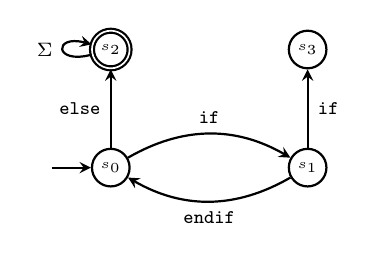
\begin{tikzpicture}[state/.style={circle, draw, thick, inner sep =
      2pt}]
    \begin{scope}[every node/.style={state}]
      \node (0) at (0,0) {\tiny $s_0$}; \node (1) at (2.5, 0) {\tiny
        $s_1$}; \node [double] (2) at (0, 1.5) {\tiny $s_2$}; \node
      (3) at (2.5, 1.5) {\tiny $s_3$};
    \end{scope}
    \begin{scope}[->, >=stealth, thick, auto]
      \draw (-0.75, 0) to (0); \draw (0) to node {\scriptsize
        $\mathtt{else}$ } (2); \draw (0) to [bend left=30] node
      {\scriptsize $\mathtt{if}$} (1); \draw (1) to [bend left=30]
      node {\scriptsize $\mathtt{endif}$} (0); \draw (2) to [loop
      left] node {\scriptsize $\Sigma$} (2); \draw (1) to node [right]
      {\scriptsize $\mathtt{if}$} (3);
    \end{scope}
  \end{tikzpicture}
  \caption{DSA for out-of-context \texttt{else}}
  \label{fig:if-else}
\end{figure}



\paragraph*{Overview of results.}
We formally present deterministic suffix-reading automata and its
semantics, quantify its size in comparison to an equivalent DFA, and
study an algorithm to construct DSAs starting from a DFA. This is in
the same spirit as in DGAs, where smaller DGAs are obtained by suppressing
states. For automata models with strings on transitions, the number of
states is not a faithful measure of the size of a DSA. As described
in~\cite{giammarresi1999deterministic} for DGAs, we consider the total-size of
a DSA which includes the number of states, edges, and the sum of label
lengths. The key contributions of this work are:
\begin{enumerate}
\item Presentation of a definition of a new kind of automaton - DSA~(Chapter~\ref{sec:new-automaton-model}).

\item Proof that DSAs accept regular languages, and nothing more.
\begin{enumerate}
  \item Every complete DFA can be seen as a DSA. 
  \item For the converse, we prove
  that for every DSA of size $k$, there is a DFA with size at most
  $2k \cdot (1 + 2 |\Sigma|)$, where $\Sigma$ is the alphabet
  (Lemma~\ref{lem:tracking-dfa-language-equivalent},
  Theorem~\ref{thm:comparing-dsa-with-dfa-dga}).
\end{enumerate}  
%  This answers the question of how small DSAs can be in comparison to
%  DFAs for a certain language : if $n$ is the size of the minimal DFA
%  for a language $L$, minimal DSAs for $L$ cannot be smaller than
%  $\frac{n}{2 \cdot (1 + 2
%    |\Sigma|)}$. 
%  When the alphabet is large, one could expect smaller sized DSAs. 
  We describe a family of languages $L_n$, with alphabet size $n$, for
  which the minimal DFA has size quadratic in $n$, whereas size of
  DSAs is a linear function of $n$ (Lemma~\ref{lem:dsa-small}).

\item We present a method to derive DSAs out of DFAs, a DFA-to-DSA
  conversion (Chapter~\ref{sec:suffix-tracking-sets}). 
  
  The derivation procedure selects subsets of DFA-states, and adds
  transitions labeled with (some of) the acyclic paths between
  them. We identify sufficient conditions on
  the selected subset of states, so that the derivation procedure
  preserves the language (Theorem~\ref{def:suffix-tracking-set}).

\item We remark that minimal DSAs need not be unique, and make an
  observation: the smallest DSA that we derive from the
  canonical DFA of a language $L$ need not be a minimal DSA. 
%  We find this
%  surprising because (1) firstly, our derivation procedure is
%  surjective: every DSA (satisfying some natural assumptions) can be
%  derived from some corresponding DFA, and in particular, a minimal
%  DSA can be derived from some DFA; (2) the observation suggests that
%  one may need to start with a bigger DFA in order to derive a minimal
%  DSA -- so, starting with a bigger DFA may result in a smaller DSA
  (Section~\ref{sec:minim-some-observ}).

\item Motivated by the above observation, we present a restricted definition of DSA, called \emph{strong DSA} (Section~\ref{sec:strong}). We show that minimal strong DSAs can in fact be derived from the canonical DFA, through our derivation procedure. 


\item Finally, we show that given a DFA and a number $k$, deciding if
  there exists a DSA of size $\le k$ is $\NP$-complete
  (Section~\ref{sec:complexity}).

\end{enumerate}

\paragraph*{Related work.} The closest to our work
is~\cite{giammarresi1999deterministic} which introduces DGAs, and
gives a procedure to derive DGAs from DFAs. The focus however is on
getting DGAs with as few states as possible. The observations presented in
Chapter~\ref{sec:minim-some-observ} of our work, also apply for
state-minimality: the same example shows that in order to get a DSA with fewer
states, one may have to start with a bigger DFA.  This is in sharp
contrast to the DGA setting, where the derivation procedure of
\cite{giammarresi1999deterministic} yields a minimal DGA (in the
number of states) when applied on the canonical DFA. The problem of
deriving DGAs with minimal total-size was left open
in~\cite{giammarresi1999deterministic}, and continues to remain so, to
the best of our knowledge.
Expression automata~\cite{DBLP:conf/wia/HanW04} allow regular
expressions as transition labels.  This model was already considered
in~\cite{DBLP:journals/tc/BrzozowskiM63} to convert automata to
regular expressions. Every DFA can be converted to a two state
expression automaton with a regular expression connecting them.  A
model of deterministic Expression automata (DEA) was proposed
in~\cite{DBLP:conf/wia/HanW04} with restrictions that limit the
expressive power.  An algorithm to convert a DFA to a DEA, by repeated
state elimination, is proposed in~\cite{DBLP:conf/wia/HanW04}. The
resulting DEA is minimal in the number of states.  
Minimization of NFAs was studied
in~\cite{DBLP:journals/siamcomp/JiangR93} and shown to be
hard. Succinctness of models with different features, like alternation,
two-wayness, pebbles, and a notion of concurrency, has been studied
in~\cite{DBLP:journals/tcs/GlobermanH96}.

Here are some works that are related to the spirit of finding more readable specifications. \cite{fernau2009algorithms} has used the model of deterministic GA to
develop a learning algorithm for some simple forms of regular
expressions, with
applications in learning DTD specifications for XML code. In this
paper, the author talks about readability of specifications. They
claim that regular expressions (REs) are arguably the best way to
specify regular 
languages. They also claim that the translation algorithms from DFAs
to REs give unreadable REs. In the paper, they consider specific
language classes and generate algorithms to learn simple looking REs.

Another work that talks about readability of specifications
is~\cite{DBLP:conf/icse/ZimmermanLL02}. They consider automata based
specification languages and perform extensive
experiments to determine which choice of syntax gives better
readability. They remark that hierarchical specifications are easier,
since not every transition needs to be specified. Once again, we
observe that there is an effort to remove transitions. Another
formalism is EDT, proposed in~\cite{DBLP:conf/date/VenkateshSKA14}, which
uses a tabular notation where each cell contains patterns, which is
then compiled into a usual automaton for analysis.



\section{Bridging the Gap to Concurrent Systems}
DSA provide a new toolkit for the succinct specification of sequential, pattern-based systems. However, modern software systems are rarely monolithic and sequential. They are typically composed of multiple interacting components that operate concurrently. This section motivates the extension of the suffix-reading paradigm from the sequential to the concurrent domain \cite{Keerthan2025netys}.

\subsection*{The Limits of Sequential Models for Concurrency}
Applying a sequential model like a DSA directly to a concurrent system runs into an obstacle: the "interleaving explosion". A concurrent system consists of multiple processes or components that execute asynchronously. To model such a system with a sequential automaton, one must account for all possible orderings, or interleavings, of the events generated by the different components. The number of such interleavings grows exponentially with the number of events.

This problem is made concrete by a Car Security System example, illustrated in Figure \ref{fig:car-example}. A practical requirement for starting a car might be that the key is in the ignition (K), the brake pedal is pressed (B), and the transmission is in park (P), with these three actions allowed to occur in any order. A standard DSA, in order to capture this behaviour, would be forced to have a transition whose label explicitly enumerates all $3! = 6$ permutations: KBP, KPB, BKP, BPK, PKB, and PBK. This approach completely undermines the goal of conciseness and readability that motivated the DSA model in the first place. As the number of concurrent components grows, this becomes utterly impractical.

\subsection*{Specification of Concurrent Suffix-Based Rules}
The failure of the sequential model in the setting of concurrency gives rise to the second central problem of this thesis: \textit{How can we model specifications that involve patterns across multiple concurrent "ports"?} A natural syntactic approach is to introduce a parallel composition operator $\parallel$, into the transition labels. Using this operator, the car security requirement could be expressed with a single, elegant transition labeled `K $\parallel$ B $\parallel$ P'. This syntax would abstract away the interleavings, capturing the logical intent of the specification directly. However, introducing such an operator should not be merely a syntactic convenience. The core challenge lies in defining a formal operational semantics for it that is both theoretically sound and intuitively useful for a wide range of real-world specification scenarios. The development of such a semantics is the primary focus of this next part.

   \begin{figure}
   \centering
   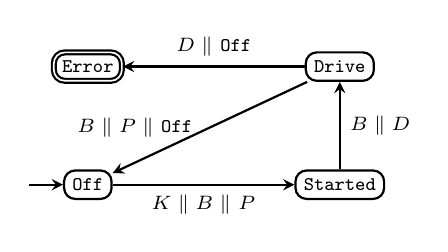
\begin{tikzpicture}
      \begin{scope}[every node/.style={rectangle, rounded corners, draw, inner sep=3pt, thick}]
        \node (0) at (0,0) {\scriptsize \texttt{Off}};
        \node [double] (1) at (0,1.5) {\scriptsize \texttt{Error}};
        \node (2) at (3.2,0) {\scriptsize \texttt{Started}};
        \node (3) at (3.2,1.5) {\scriptsize \texttt{Drive}};
      
      \end{scope}

      \begin{scope}[->,>=stealth, thick, auto]
        \draw (-0.75,0) to (0);
        %\draw (0) to [bend left] node [left] {\scriptsize \texttt{On}} (1);
        %\draw (1) to [bend left] node [right] {\scriptsize \texttt{Off}} (0);
        \draw (0) to node [below] {\scriptsize $K \parallel B \parallel$ $P$} (2);
        \draw (2) to node [right] {\scriptsize $B \parallel D$ } (3);
        \draw (3) to node [left] {\scriptsize $B \parallel P \parallel$ \texttt{Off}$~$} (0); 
        \draw (3) to node [above] {\scriptsize $D \parallel$ \texttt{Off}} (1);
      \end{scope}
   \end{tikzpicture}
   \caption{Car security system example}
   \label{fig:car-example}
   \end{figure}


\paragraph*{Our model.}
To address the challenge of specifying concurrent systems, this thesis introduces the \textbf{Multi-port Suffix-reading Automaton (mDSA)}, an extension of the DSA model designed to handle concurrency and outputs. 

The mDSA model operates over a multi-port alphabet $\Sigma = \langle\Sigma_1, ..., \Sigma_k\rangle$, where the global alphabet is partitioned among $k$ distinct ports. Transitions are labeled with concurrent patterns like $(u_1 \parallel u_2 \parallel ... \parallel u_k)$, where each $u_i$ is a word (a pattern) from the alphabet of port $i$, $\Sigma_i^*$ \cite{Keerthan2025netys}.

%The key idea of the mDSA model lies in its operational semantics, which is defined over a configuration that explicitly manages the system's history. An mDSA configuration is a tuple $(q, w, \Theta)$, where:
%\begin{itemize}
%    \item $q$ is the current state of the automaton.
%    \item $w$ represents the persistent history of input symbols received by the system across all ports.
%    \item $\Theta$ is a numerical marker, or "tape head," indicating the position in the history string $w$ where the last successful transition match occurred.
%\end{itemize}
%This configuration structure allows for a matching rule that resolves a fundamental dilemma in event-based specification. The dilemma, highlighted by contrasting a car security system (which needs to remember that a brake pedal is still pressed) with a smartphone lock (which needs to detect a fresh button press), is whether to consume input history or not. Consuming it loses context, while not consuming it can lead to infinite loops on old data.
%
%The $(q, w, \Theta)$ mechanism solves this. A concurrent transition $(u_1 \parallel ... \parallel u_k)$ is defined to match a tape configuration $(w, \Theta)$ if two conditions hold:
%\begin{enumerate}
%    \item \textbf{Suffix Match:} For each port $i$, the pattern $u_i$ must be a suffix of that port's projected history, $P_i(w)$.
%    \item \textbf{Freshness Condition:} Critically, at least one of the patterns $u_i$ must have occurred entirely after the marker $\Theta$. That is, its corresponding subword in $w$ must lie completely within $w[\Theta+1, |w|]$.
%\end{enumerate}
%This marker provides a formal and precise mechanism for capturing the intuitive notion of a "fresh event." It allows the model to check for both persistent conditions (patterns that occurred before $\Theta$) and new trigger events (patterns that occurred after $\Theta$), accommodating both types of specification scenarios within a single, coherent semantic framework.


The development of the mDSA model is not just theoretical, but driven by the practical need to formalize existing industrial specification methods. This is demonstrated through its application to {Expressive Decision Tables (EDTs)}~\cite{DBLP:conf/date/VenkateshSKA14}, a tabular notation used successfully in industry for specifying the requirements of reactive systems. EDTs allow engineers to specify complex, suffix-based rules in a convenient format. For example, a particular rule in a safety system might specify that if the `Panic Switch' were pressed twice while the `Alarm' is `Off', an error should be generated. (shown as a DSA in Figure \ref{fig:alarm-example})

  \begin{figure}
  \centering
  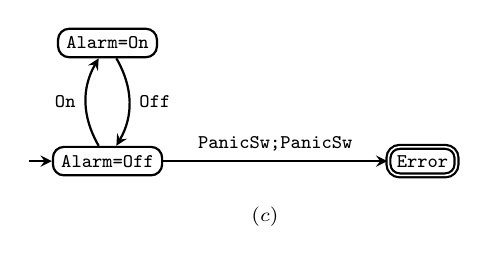
\begin{tikzpicture}[state/.style={circle, inner sep=2pt, draw, thick}]
    \begin{scope}%[every node/.style={state}]

        \begin{scope}
          \node [rectangle, rounded corners, draw, inner sep=3pt, thick] (0) at (0,0) {\scriptsize \texttt{Alarm=Off}};
          \node [rectangle, rounded corners, draw, inner sep=3pt, thick] (1) at (0,1.5) {\scriptsize \texttt{Alarm=On}};
          \node [rectangle, rounded corners, draw, inner sep=3pt, thick, double] (2) at (4, 0) {\scriptsize \texttt{Error}};
        \end{scope}

        \begin{scope}[->, >=stealth, thick]
          \draw (-1,0) to (0);
          \draw (0) to [bend left] node [left] {\scriptsize \texttt{On}} (1);
          \draw (1) to [bend left] node [right] {\scriptsize \texttt{Off}} (0);
          \draw (0) to node [above] {\scriptsize \texttt{PanicSw;PanicSw}} (2);
        \end{scope}
        \node at (2, -0.7) {\scriptsize $(c)$};
      \end{scope}
    
  \end{tikzpicture}
  \caption{Panic-switch and Alarm example}
  \label{fig:alarm-example}
  \end{figure}


Despite their practical success and use in test generation, EDTs have lacked a rigorous, formal operational semantics. This gap has meant that test generation tools for EDTs often rely on heuristics and random generation, without the ability to formally prove properties or guarantee coverage. To model the full behaviour of EDTs, which includes not just input conditions but also the generation of output actions, the mDSA model requires an additional extension. This practical requirement directly motivates our development of \textbf{mDSAs-with-outputs}.

 In this model, a transition can now specify that upon matching an input condition, a set of output symbols should be produced. It creates a feedback loop where the automaton can modify input conditions of subsequent transitions via previous outputs. The main theoretical result here is that state reachability for mDSAs-with-outputs is {PSPACE-complete} \cite{Keerthan2025netys}.

%The source of this high computational complexity is illustrated using an N-bit counter example. This example shows how a polynomially-sized mDSA-with-outputs can use the input-output feedback loop to simulate a binary counter. The state of the counter is not stored in the automaton's finite state control but is instead encoded on the history tape $w$. Each increment of the counter is performed by a transition that reads the current bits from the tape and writes the new bits back to the tape. To reach the final state of the counter requires a number of steps exponential in the number of bits (N). This demonstrates that a witness for reachability can be exponentially long, leading to the PSPACE complexity.

This entire development arc embodies the (sub)title of this dissertation, "Putting Practice into Theory (and Back)." The practical need to provide a formal semantics for an industrial notation (EDT) led to theoretical model extensions, from DSA to mDSA and mDSAs-with-outputs). The formal analysis of these new theoretical models, in turn, revealed a fundamental complexity result. This theoretical discovery then feeds back to practice, providing a formal explanation for the inherent difficulty of test generation for EDT-like specifications and informing the design of such verification tools.

\section{Thesis Contributions and Outline}
This dissertation introduces and analyzes a new family of automata, Suffix-Reading Automata, designed to provide succinct and readable formal models for sequential and concurrent systems. The research bridges the gap between automata theory and engineering practice by developing formalisms that are both theoretically sound and practically motivated.

\subsection*{Summary of Contributions}
The primary contributions of this dissertation can be summarized as follows:
\begin{itemize}
    \item \textbf{A Model for Sequential Specifications:} The introduction of the Deterministic Suffix-reading Automaton (DSA) as a novel, fully expressive, and deterministic formalism for regular languages. This model provides a more succinct and readable representation for pattern-intensive specifications compared to traditional DFAs. A theoretical analysis of its properties is provided.
    \begin{itemize}
    	\item \textbf{Automaton Minimization Analysis:} The discovery of a fundamental bottleneck in DSA minimization, demonstrating that the canonical (Myhill-Nerode) DFA is insufficient for deriving minimal DSAs. This is complemented by a formal proof that the DSA minimization problem is NP-complete. As a constructive solution, the Strong DSA (sDSA) subclass is introduced, which is shown to be a tractable and well-behaved class for which minimal automata are derivable from the canonical DFA.
    \end{itemize}
    
    \item \textbf{A Model for Concurrent Specifications:} The extension of the suffix-reading paradigm to concurrent systems with the Multi-port DSA (mDSA). This model features a tape-based semantics with a history marker that formalizes the management of event history and the notion of "freshness" required for triggering concurrent transitions.
    \begin{itemize}
    	\item \textbf{Bridging Formalism and Industrial Practice:} The development of the first formal operational semantics for the industrial Expressive Decision Table (EDT) notation, via a translation to mDSAs-with-outputs. The proof that the associated test generation problem (state reachability) is PSPACE-complete reveals the complexity inherent in such practical specification languages.
    \end{itemize}
\end{itemize}

\subsection*{Thesis Structure}
The remainder of this dissertation is organized as follows:
\begin{itemize}
    \item \textbf{Chapter 2: Preliminaries (with a Survey of Automata Models):} This chapter will formally define the foundational concepts from automata theory and formal methods that are used throughout the thesis. It will also present a technical introduction of related automata models discussed in this introduction.
    \item \textbf{Chapter 3: Deterministic Suffix-Reading Automata (DSA):} This chapter will present the formal definition, semantics and theoretical analysis of the DSA model. This includes proofs of expressiveness, and succinctness results.
    \item \textbf{Chapter 4: Derivation of DSAs:} This chapter will detail the DFA-to-DSA derivation procedure via suffix-tracking sets.
    \item \textbf{Chapter 4: DSA Minimality:} This chapter will demonstrate the canonical DFA bottleneck for minimization, the full NP-completeness proof, and the theory of Strong DSAs (sDSAs).
    \item \textbf{Chapter 6: Multi-Port DSA (mDSA):} This chapter will introduce the mDSA model for specifying concurrent systems. It will detail the multi-port alphabet, the $\parallel$ operator, and the tape-based semantics.
    \item \textbf{Chapter 7: Application to Expressive Decision Tables (mDSA-with-outputs):} This chapter will present the translation from the EDT notation to mDSAs-with-outputs. It will then present the full proof of PSPACE-completeness for the state reachability problem.
    \item \textbf{Chapter 8: Conclusion and Future Work:} This chapter will summarize the key findings of the dissertation and discuss several promising directions for future research.
\end{itemize}

%\section{Comments}
%
%After 1.1 and 1.2, section 1.3 can be ``Contributions of this thesis''. Within this there can be five subsections: DSA, Challenges, Gap to Concurrent systems, Multi-port DSA, Summary.
%
%Goal is to get a technical summary of the entire thesis. Examples need to be there and the main theorems should be highlighted. State the theorems (use restatable)
%
%Put EDTs before starting the technical summary of the thesis. The challenges with EDT: wanted to test generation, and first needed a formal model of it. 

